\documentclass[14pt]{extbook}
\usepackage{multicol, enumerate, enumitem, hyperref, color, soul, setspace, parskip, fancyhdr} %General Packages
\usepackage{amssymb, amsthm, amsmath, latexsym, units, mathtools} %Math Packages
\everymath{\displaystyle} %All math in Display Style
% Packages with additional options
\usepackage[headsep=0.5cm,headheight=12pt, left=1 in,right= 1 in,top= 1 in,bottom= 1 in]{geometry}
\usepackage[usenames,dvipsnames]{xcolor}
\usepackage{dashrule}  % Package to use the command below to create lines between items
\newcommand{\litem}[1]{\item#1\hspace*{-1cm}\rule{\textwidth}{0.4pt}}
\pagestyle{fancy}
\lhead{Progress Quiz 9}
\chead{}
\rhead{Version B}
\lfoot{9541-5764}
\cfoot{}
\rfoot{Summer C 2021}
\begin{document}

\begin{enumerate}
\litem{
Construct the lowest-degree polynomial given the zeros below. Then, choose the intervals that contain the coefficients of the polynomial in the form $ax^3+bx^2+cx+d$.\[ \frac{5}{2}, \frac{-1}{2}, \text{ and } -7 \]\begin{enumerate}[label=\Alph*.]
\item \( a \in [2, 10], b \in [36.1, 42.5], c \in [86, 95], \text{ and } d \in [30, 40] \)
\item \( a \in [2, 10], b \in [18.8, 21.8], c \in [-65, -58], \text{ and } d \in [-35, -32] \)
\item \( a \in [2, 10], b \in [35.9, 37.2], c \in [42, 60], \text{ and } d \in [-35, -32] \)
\item \( a \in [2, 10], b \in [-22.7, -19.9], c \in [-65, -58], \text{ and } d \in [30, 40] \)
\item \( a \in [2, 10], b \in [18.8, 21.8], c \in [-65, -58], \text{ and } d \in [30, 40] \)

\end{enumerate} }
\litem{
Describe the end behavior of the polynomial below.\[ f(x) = -6(x - 6)^{3}(x + 6)^{6}(x + 2)^{3}(x - 2)^{3} \]\begin{enumerate}[label=\Alph*.]
\begin{multicols}{2}\item 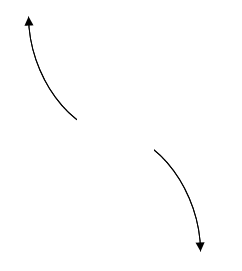
\includegraphics[width = 0.3\textwidth]{../Figures/polyEndBehaviorCopyAB.png}\item 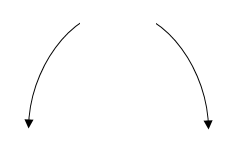
\includegraphics[width = 0.3\textwidth]{../Figures/polyEndBehaviorCopyBB.png}\item 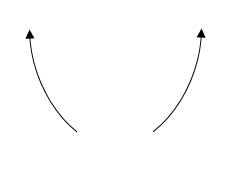
\includegraphics[width = 0.3\textwidth]{../Figures/polyEndBehaviorCopyCB.png}\item 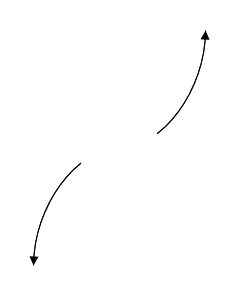
\includegraphics[width = 0.3\textwidth]{../Figures/polyEndBehaviorCopyDB.png}\end{multicols}\item None of the above.
\end{enumerate} }
\litem{
Construct the lowest-degree polynomial given the zeros below. Then, choose the intervals that contain the coefficients of the polynomial in the form $x^3+bx^2+cx+d$.\[ 4 - 3 i \text{ and } 2 \]\begin{enumerate}[label=\Alph*.]
\item \( b \in [-15, -8], c \in [35, 44], \text{ and } d \in [-50, -44] \)
\item \( b \in [-5, 4], c \in [1, 7], \text{ and } d \in [-8, 2] \)
\item \( b \in [10, 15], c \in [35, 44], \text{ and } d \in [50, 56] \)
\item \( b \in [-5, 4], c \in [-9, 0], \text{ and } d \in [6, 11] \)
\item \( \text{None of the above.} \)

\end{enumerate} }
\litem{
Which of the following equations \textit{could} be of the graph presented below?
\begin{center}
    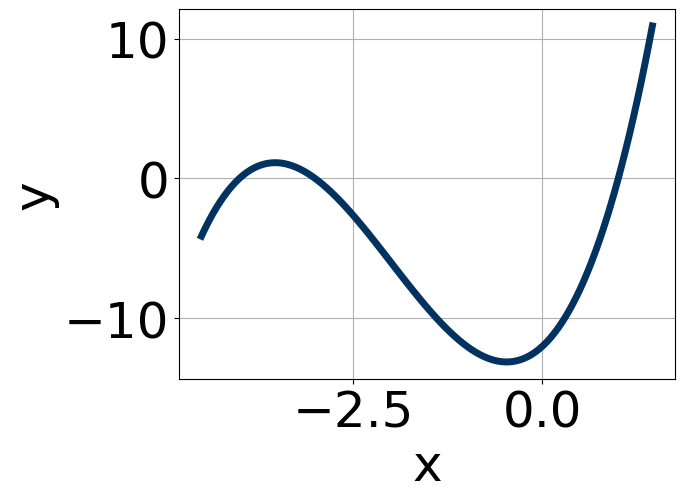
\includegraphics[width=0.5\textwidth]{../Figures/polyGraphToFunctionCopyB.png}
\end{center}
\begin{enumerate}[label=\Alph*.]
\item \( 15(x - 1)^{4} (x + 3)^{4} (x + 4)^{9} \)
\item \( -12(x - 1)^{10} (x + 3)^{11} (x + 4)^{11} \)
\item \( -11(x - 1)^{11} (x + 3)^{7} (x + 4)^{7} \)
\item \( 3(x - 1)^{7} (x + 3)^{9} (x + 4)^{9} \)
\item \( 20(x - 1)^{8} (x + 3)^{5} (x + 4)^{9} \)

\end{enumerate} }
\litem{
Describe the zero behavior of the zero $x = 4$ of the polynomial below.\[ f(x) = -6(x - 4)^{2}(x + 4)^{3}(x - 8)^{2}(x + 8)^{5} \]\begin{enumerate}[label=\Alph*.]
\begin{multicols}{2}\item 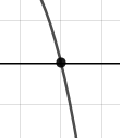
\includegraphics[width = 0.3\textwidth]{../Figures/polyZeroBehaviorCopyAB.png}\item 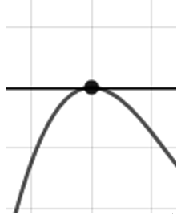
\includegraphics[width = 0.3\textwidth]{../Figures/polyZeroBehaviorCopyBB.png}\item 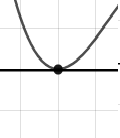
\includegraphics[width = 0.3\textwidth]{../Figures/polyZeroBehaviorCopyCB.png}\item 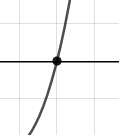
\includegraphics[width = 0.3\textwidth]{../Figures/polyZeroBehaviorCopyDB.png}\end{multicols}\item None of the above.
\end{enumerate} }
\litem{
Describe the zero behavior of the zero $x = 5$ of the polynomial below.\[ f(x) = -5(x + 5)^{3}(x - 5)^{4}(x + 7)^{2}(x - 7)^{4} \]\begin{enumerate}[label=\Alph*.]
\begin{multicols}{2}\item 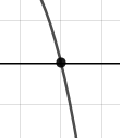
\includegraphics[width = 0.3\textwidth]{../Figures/polyZeroBehaviorAB.png}\item 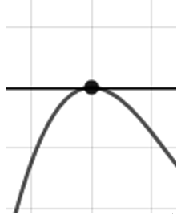
\includegraphics[width = 0.3\textwidth]{../Figures/polyZeroBehaviorBB.png}\item 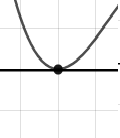
\includegraphics[width = 0.3\textwidth]{../Figures/polyZeroBehaviorCB.png}\item 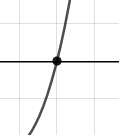
\includegraphics[width = 0.3\textwidth]{../Figures/polyZeroBehaviorDB.png}\end{multicols}\item None of the above.
\end{enumerate} }
\litem{
Describe the end behavior of the polynomial below.\[ f(x) = 6(x - 6)^{4}(x + 6)^{7}(x - 5)^{3}(x + 5)^{4} \]\begin{enumerate}[label=\Alph*.]
\begin{multicols}{2}\item 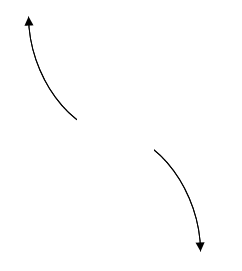
\includegraphics[width = 0.3\textwidth]{../Figures/polyEndBehaviorAB.png}\item 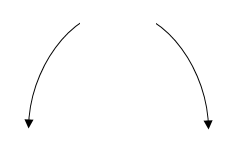
\includegraphics[width = 0.3\textwidth]{../Figures/polyEndBehaviorBB.png}\item 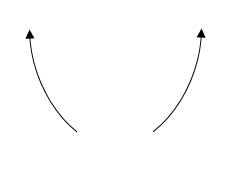
\includegraphics[width = 0.3\textwidth]{../Figures/polyEndBehaviorCB.png}\item 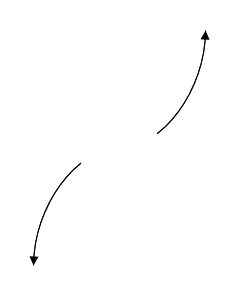
\includegraphics[width = 0.3\textwidth]{../Figures/polyEndBehaviorDB.png}\end{multicols}\item None of the above.
\end{enumerate} }
\litem{
Construct the lowest-degree polynomial given the zeros below. Then, choose the intervals that contain the coefficients of the polynomial in the form $x^3+bx^2+cx+d$.\[ -3 - 4 i \text{ and } 1 \]\begin{enumerate}[label=\Alph*.]
\item \( b \in [-2.7, 4.7], c \in [0.81, 2.83], \text{ and } d \in [-3.5, -2.56] \)
\item \( b \in [-7.9, -3.5], c \in [17.28, 19.46], \text{ and } d \in [24.68, 25.62] \)
\item \( b \in [-2.7, 4.7], c \in [2.24, 5.06], \text{ and } d \in [-4.56, -3.05] \)
\item \( b \in [3.6, 7.4], c \in [17.28, 19.46], \text{ and } d \in [-25.02, -24.7] \)
\item \( \text{None of the above.} \)

\end{enumerate} }
\litem{
Construct the lowest-degree polynomial given the zeros below. Then, choose the intervals that contain the coefficients of the polynomial in the form $ax^3+bx^2+cx+d$.\[ \frac{-2}{3}, \frac{1}{3}, \text{ and } \frac{5}{4} \]\begin{enumerate}[label=\Alph*.]
\item \( a \in [35, 37], b \in [-38, -31], c \in [-31, -22], \text{ and } d \in [-13, -7] \)
\item \( a \in [35, 37], b \in [-38, -31], c \in [-31, -22], \text{ and } d \in [8, 17] \)
\item \( a \in [35, 37], b \in [-60, -55], c \in [4, 16], \text{ and } d \in [8, 17] \)
\item \( a \in [35, 37], b \in [-86, -76], c \in [53, 57], \text{ and } d \in [-13, -7] \)
\item \( a \in [35, 37], b \in [32, 39], c \in [-31, -22], \text{ and } d \in [-13, -7] \)

\end{enumerate} }
\litem{
Which of the following equations \textit{could} be of the graph presented below?
\begin{center}
    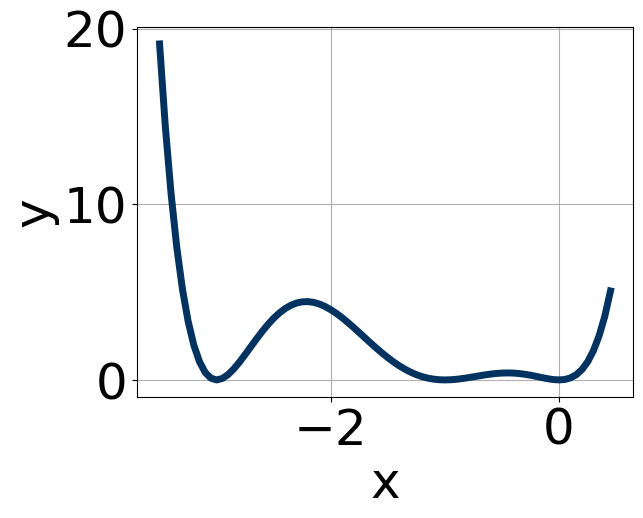
\includegraphics[width=0.5\textwidth]{../Figures/polyGraphToFunctionB.png}
\end{center}
\begin{enumerate}[label=\Alph*.]
\item \( 4x^{10} (x + 3)^{10} (x + 1)^{6} \)
\item \( 10x^{8} (x + 3)^{8} (x + 1)^{11} \)
\item \( 6x^{5} (x + 3)^{4} (x + 1)^{9} \)
\item \( -15x^{10} (x + 3)^{4} (x + 1)^{10} \)
\item \( -6x^{6} (x + 3)^{8} (x + 1)^{5} \)

\end{enumerate} }
\end{enumerate}

\end{document}